\chapter{Introducción a FreeCAD}

\begin{figure}[H]
	\centering
	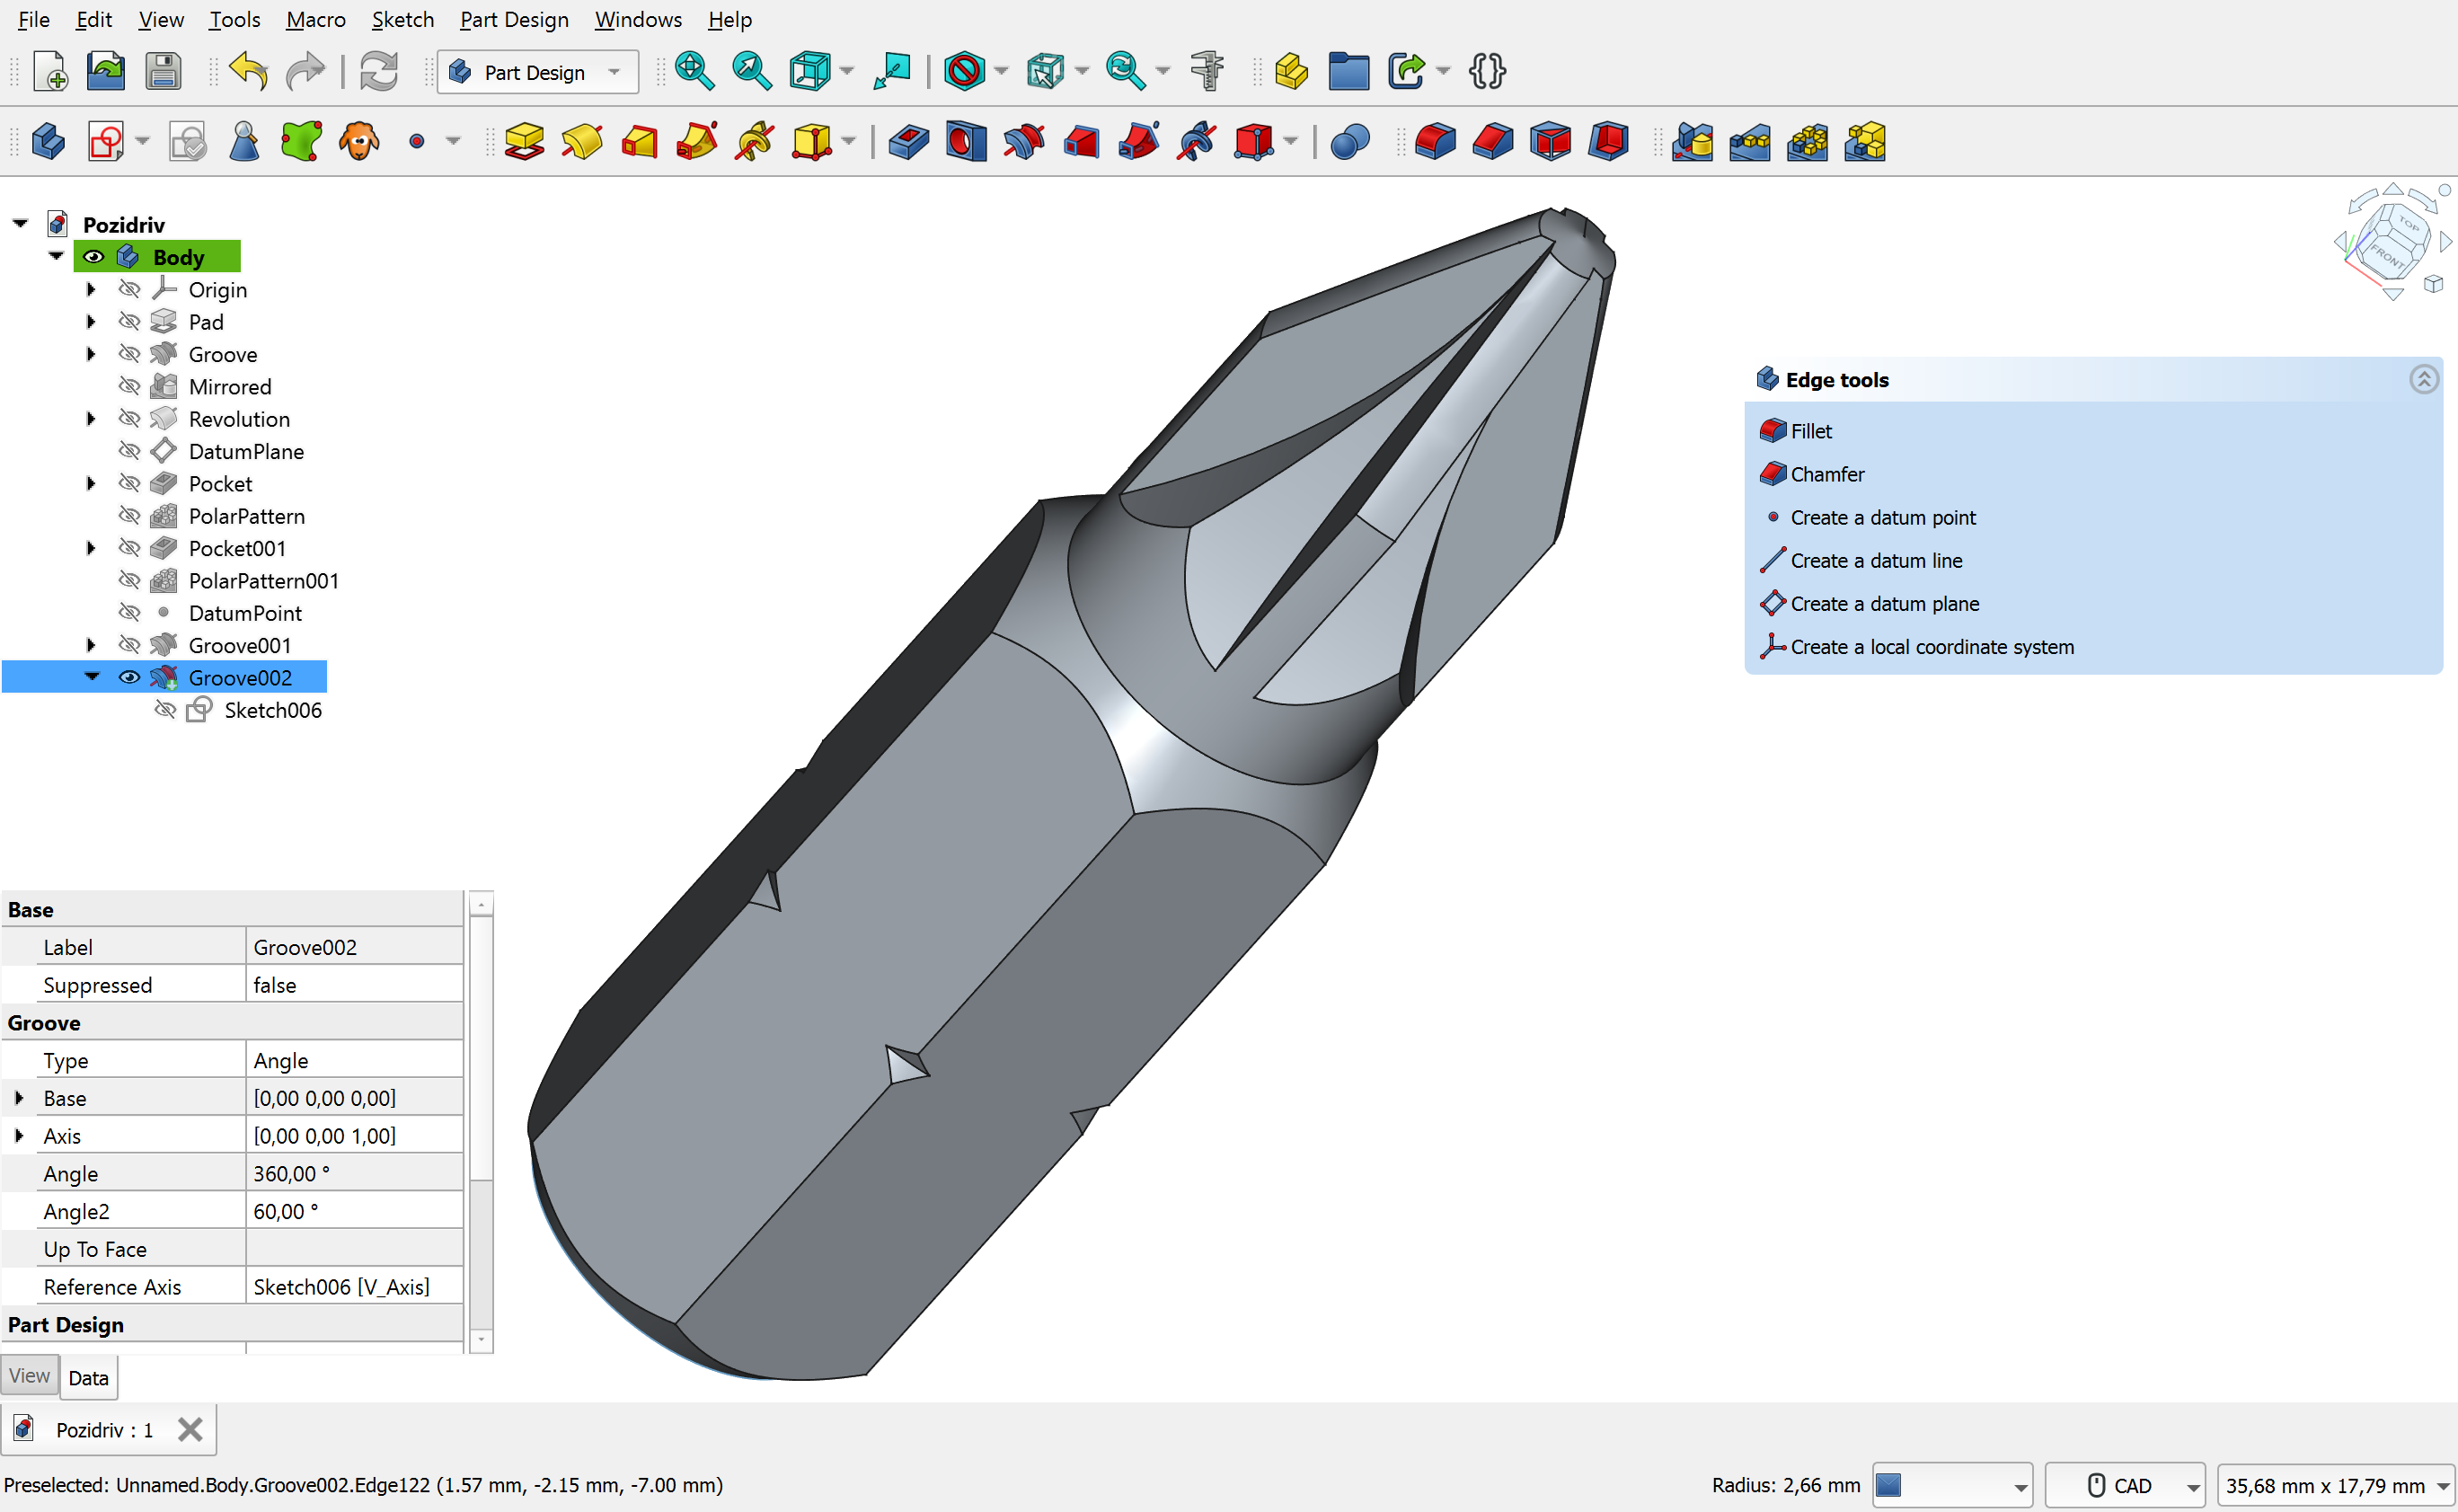
\includegraphics[width=0.8\textwidth]{img/cap1_freecad.png}
	\caption{Interfaz principal de FreeCAD con el módulo Part Design activo}
\end{figure}

FreeCAD es un software de diseño asistido por computadora (CAD)
3D de código abierto y gratuito. Permite crear modelos
paramétricos para ingeniería, arquitectura y fabricación.

%% D. Búsqueda e Inserción de Activos Gráficos
%% Imagen insertada al inicio del capítulo

%% B. Actividades Teóricas
\section{Investigar y responder}
\faPencil

Investiga sobre FreeCAD y responde:
\begin{enumerate}
	\item ¿Qué significa que FreeCAD sea de código abierto?
	\item ¿Cuáles son las principales ventajas del modelado
	      paramétrico?
	\item ¿Qué formatos de archivo puede importar y exportar
	      FreeCAD?
	\item ¿Qué lenguaje de programación se utiliza para
	      extender FreeCAD?
	\item ¿Por qué es importante usar software libre en la
	      educación técnica?
	\item Nombra tres industrias donde se utiliza FreeCAD
	      actualmente.
	\item ¿Qué diferencia a FreeCAD de otros programas CAD
	      comerciales?
	\item ¿Cuál es la licencia bajo la cual se distribuye
	      FreeCAD?
\end{enumerate}

%% C. Actividades Prácticas
\section{Resolver los siguientes problemas}
\faWrench

Problemas para aplicar conocimientos:
\begin{enumerate}
	\item Instala FreeCAD en tu computadora y verifica que
	      funcione correctamente.
	\item Localiza en la interfaz las barras de herramientas
	      principales.
	\item Abre y cierra tres archivos de ejemplo que trae
	      FreeCAD.
	\item Exporta un archivo a formato STL.
	\item Cambia el idioma de la interfaz a español.
	\item Configura el tema de color oscuro en las preferencias.
	\item Busca documentación oficial de FreeCAD en español.
	\item Identifica los workbenches disponibles en tu versión.
	\item Realiza una captura de pantalla de la interfaz y
	      anota los elementos principales.
	\item Comparte con un compañero las características
	      principales de FreeCAD.
\end{enumerate}